\documentclass[10pt]{article}
\title{Math 1551, Differential Calculus Worksheets}
\author{}

% LOAD PACKAGES
\usepackage{amsmath} % allows for align env and other things
\usepackage{graphicx} % allows for graphics
\usepackage{textcomp} % allows for single apostrophe
\usepackage{enumitem} % allows for alpha lettering in enumerated lists
\usepackage{amsfonts} % for real numbers symbol and other sets
\usepackage[mathscr]{euscript} % Euler script font
\usepackage{wrapfig} % to allow text wrapping
\usepackage{pgfplots} % for tikz graphics

% FONT FORMAT
\renewcommand*\rmdefault{ppl} % change font to Palatino

% MARGINS
\usepackage{anysize}
\marginsize{2.5cm}{2.5cm}{2cm}{3cm}

% SHORTCUTS
\newcommand{\Textbook}{Thomas 13$^{th}$ Edition}
\newcommand{\Sections}{Sections from \Textbook: }


\newcommand{\SolutionsStatement}{As stated in the syllabus, a goal of this course is to prepare students for more advanced courses that have this course as a pre-requisite. To help us meet this goal, the solutions that are provided for worksheets only give what you would need to write in a quiz, midterm or exam. This is intentional: upper level math courses often don't have recitations, let alone worksheets and worksheet solutions. So students need, develop, and use various strategies to check their solutions in those courses. \\[6pt]

In this course, students are encouraged to ask questions they may have about the course on Piazza, office hours, by checking their answers with their peers, or by asking their instructor after class or over email. Calculators and software are also great ways to check your work. All of these methods are valuable skills that are transferable to higher level courses.}

\newcommand{\Course}{Math 1551}
\newcommand{\Semester}{Spring 2017}
\newcommand{\TorF}{Indicate whether the statement true or false. If it is true, in one or two sentences, explain why. If false, give a counter example or explain why in one or two sentences.}

\newcommand{\TorFShort}{Indicate whether the statement true or false. Explain your reasoning.}

% OTHER
\newcommand{\R}{{\mathbb R}} % The real numbers
\newcommand{\Emph}[1]{\textbf{#1}} % Emphasize

% DERIVATIVES
\newcommand{\dfdx}{\frac{df}{dx}}
\newcommand{\dfdt}{\frac{df}{dt}}
\newcommand{\ddx}{\frac{d}{dx}}
\newcommand{\ddt}{\frac{d}{dt}}
\newcommand{\dxdt}{\frac{dx}{dt}}
\newcommand{\dydt}{\frac{dy}{dt}}

% FANCY HEADERS
%\usepackage{fancyhdr}
%\pagestyle{fancy}
%\fancyhf{}
%\date{}
%\lhead{Please print first and last names: }
%\rhead{Worksheet for \thesection\hspace{0.25cm}}

%\usepackage{lastpage} % for fancy page numbering
%\rfoot{Page \thepage \hspace{1pt} } %of \pageref{LastPage}}

% REMOVE FIRST LINE INDENTATION 
\setlength\parindent{0pt}


% ~ ~ ~ ~ ~ ~ ~ ~ ~ ~ ~ ~ ~ ~ ~ ~ ~ ~ ~ ~ ~ ~ ~ 
\begin{document}
%\input{FrontPage.tex}

%\setcounter{section}{05}


%\newpage\section*{Worksheet 1, \Course, \Semester} 
\noindent \Sections 1.1, 1.2, 1.3

\subsection*{Welcome to Math 1551 Recitation!} 
    
    Recitations are meant for students to complete additional exercises, with a TA and other students, on topics recently covered in lecture. Recitations are meant to be
    \begin{itemize}
        \item active: students should be solving exercises themselves during recitations
        \item collaborative: students are encouraged to work together during recitation, to present their solutions on the board, and to ask for help from the TA
    \end{itemize}

Each worksheet provides exercises for one recitation.
    \begin{itemize}
        \item There may not be time in recitation to complete all exercises. 
        \item Students are expected to be able to solve all worksheet exercises.
    \end{itemize}
    
    Students are also encouraged to seek help from TAs, their instructor, and other students if they have any questions on any of the worksheet exercises. All questions are numbered, so students can more easily refer to them outside of recitation, in Piazza, in office hours, and so on.

\subsection*{Background Review}
\begin{itemize}
	\item \emph{Function $y = f(x)$}: a rule that assigns each value of $x$ to exactly one value of $y$.
	\item \emph{Domain of a function $f(x)$}: all the values that $x$ can have. 
	\item \emph{Range of a function $f(x)$}: all the values that $f(x)$ can have. 
	\item \emph{Composite function}: we define $(f \circ g)(x) = f (g(x))$.
\end{itemize}

You should be able to graph the functions below.
\vspace{-6pt}
\begin{center}
	\def\arraystretch{1.5}
    \begin{tabular}{ p{3cm} p{3cm} p{3cm} p{6cm} }
        $y = mx + b$ & $y = x^2$ & $y = x^3$ & $y=x^n$, $n$ any integer \\
        $y = |x|$ & $y=\sqrt{x}$ & $\sqrt{1 - x^2}$ & $\frac{1}{x}$\\
        $\sin x$ & $\cos x$ & $\tan x$ & $\csc x$ \\
        $\sec x$ & $\cot x$ 
    \end{tabular}
\end{center}

You should also be able to graph transformations of the above functions. Recall the following basic transformations:
\begin{itemize}
	\item \emph{Vertical shift}: $y = f(x) + c$ shifts up or down $c$ units
    \item \emph{Horizontal shift}: $y = f (x - c)$ shifts left or right $c$ units.
    \item \emph{Reflections}: $y = −f(x)$ reflects about the $x$-axis and $y = f(−x)$ reflects about the $y$-axis. 
    \item \emph{Stretching/Compressing}: $y = af(x)$ stretches when $|a| > 1$ and compresses when $0 < |a| < 1$; $y = f(bx)$ stretches when $0 < |b| < 1$ and compresses when $|b| > 1$.
\end{itemize}

\newpage
\subsection*{Trigonometric Identities}

Pythagorean Identities

$$\sin^2 x + \cos^2 x = 1, \qquad 1 + \tan^2 x = \sec^2 x, \qquad 1 + \cot^2 x = \csc^2 x$$

Half-Angle Formulas
$$\sin^2 x = \frac{1}{2}[1 - \cos(2x)] , \qquad \cos^2 x = \frac{1}{2} [1 + \cos(2x)] $$

Double-Angle Formulas
$$\sin(2x) = 2 \sin x \cos x $$ $$ \cos(2x) =\cos^2 x - \sin^2 x = 1 - 2 \sin^2 x
= 2 \cos^2 x - 1$$

Angle Sum and Difference
$$\sin (x \pm y) = \sin x \cos y \pm \sin y \cos x $$ 
$$\cos (x \pm y) = \cos x \cos y \mp \sin y \sin x $$

\subsection*{Exercises}

\begin{enumerate}
	\item Identify the domain and range of the following functions and sketch them. 
    \begin{enumerate}
    	\item $\displaystyle{f(u) = \sqrt{25 - u^2}-1}$
        \item $g(t) = t^2 -8t + 3$
        \item $A(x) = \begin{cases} 
      \displaystyle{1+\frac{1}{x-1}} & x\leq 0 \\[8pt]
      \displaystyle{\sqrt{4 - x^2}} & 0 < x\leq 2 \\
   \end{cases}$
    \end{enumerate}
	\item Given that $\sec \theta = -\sqrt{2}$, and that $\theta \in [\pi,3\pi/2]$, compute the values of the other five trig functions.
    \item If possible, give at least one example of a function for each of the following cases.
    \begin{enumerate}
    	\item A function that is decreasing for all values of $x$ and whose range is the interval $(0,\infty)$.
        \item A non-constant even function whose range is the interval $[0,1]$.
        \item A function, $f(x)$, so that $f \circ g = (x+3)(x-3)$, where $g = x^2 - 10$.
    \end{enumerate}
    \item Express $y(t)$ as a single sine function $y(t) = \frac{\sqrt{3}}{2}\cos(t) + \frac{1}{2}\sin(t)$
    \item Find all values of $\theta$ that satisfy $\sin2\theta-\cos\theta = 0$.
\end{enumerate}
%\newpage\subsection*{Answers}

\SolutionsStatement

\begin{enumerate}
	
    \item 
    \begin{enumerate}
    	\item We need $25-u^2 \ge 0$, so the domain is $u \in [-5,5]$. For the range, $\sqrt{25-u^2}$ is between 0 and 5, so $f(u)$ is between $-1$ and $4$. The range is the interval $[-1,4]$. 
        \item Complete the square: $t^2 - 8t +3 = t^2 - 8t +16 - 16 +3 = (t-4)^2 - 13$. The domain is the set of real numbers, and the range is the interval $[-13,\infty)$.
        \item $1+\frac{1}{x - 1}$ is defined for $x \le 0$ and $\sqrt{4 - x^2}$ is defined on $(0,2]$. So the domain of $A$ is the interval $(-\infty,2]$. Range: $[0,2)$. 
    \end{enumerate}

	\begin{center}
		\includegraphics[width=0.8\textwidth]{images/imgWS1Spring17.png} 
	\end{center}

	\item If $\sec \theta = -\sqrt{2}$, then $\cos\theta = -1/\sqrt{2}$, so $\theta = 5\pi/4$. 
    \begin{align*}
    	\cos 5\pi/4 &= -1/\sqrt{2} \\
        \sin 5\pi/4 &= -1/\sqrt{2} \\
        \csc 5\pi/4 &= -\sqrt{2} \\
        \tan 5\pi/4 &= 1 \\
        \cot 5\pi/4 &= 1
    \end{align*}
    \item The purpose of this question to help students become familiar with properties of elementary and rational functions.
    	\begin{enumerate} 
    		\item $2^{-x}$, or $a^{-x}$ for any $a > 0$. 
            \item $|\cos(x)|$, or $|\cos(a x)|$ for any non-zero $a$.
            \item $f(x) = x + 1$.
        \end{enumerate}
       \item Use the identity $\sin (x + y) = \cos x \sin y + \cos y \sin x$. 
       \begin{align*}
       		y &= \frac{\sqrt{3}}{2}\cos(t) + \frac{1}{2}\sin(t) \\
            &= \cos t \sin \frac{\pi}{3} + \cos \frac{\pi}{3} \sin(t) \\
            &= \sin (t + \pi / 3)
       \end{align*}
       \item \begin{align*}
        0 &= \sin2\theta-\cos\theta \\
        &= 2\cos \theta \sin\theta - \cos\theta \\
        &= \cos \theta (2\sin\theta -1)
       \end{align*}
       So either $\cos\theta = 0$ which implies $\theta = \pi/2 + n\pi$, or $\sin\theta = 1/2$, which implies $\theta = \pi/6 + 2n\pi$ and $\theta = 5\pi/6 + 2n\pi$, $n$ is any integer.
       
       
       
       
       
\end{enumerate}

%\newpage\section*{Worksheet 2, \Course, \Semester} 
\noindent \Sections 1.5, 1.6
\subsection*{Exercises}


\begin{enumerate}
	\item If possible, give at least one example of a function for each of the following cases.
    \begin{enumerate}
    	\item An odd function that not have an inverse on the domain $[-1,1]$.
        \item An even function that is invertible on the domain $[-1,1]$.
    \end{enumerate}
    \item State the domain and range of the functions.  
    \begin{enumerate}
    	\item $\ln (25 - x^2)$
        \item $\cos^{-1} (\cos x)$
        \item $\cos (\cos^{-1} x)$
    \end{enumerate}
	\item Solve for $t$. 
    	\begin{enumerate}
        	\item $3^{t+1} = r$, where $r$ is any real number
            \item $\ln t + \ln (t+1) = 1$
            \item $\log_2 (\log_3 ( \log_4 t)) = m$
            \item $2^t+2^{-t} = \frac{17}{4}$
		\end{enumerate}
     \item Find the inverse of $f(x)$. $$f(x) = \frac{e^{2x} -1}{e^{2x} + 1}$$
     \item Identify the points where $f(x) = 4^x$ and $g(x) = 2^{-x^2}$ intersect. 
     \item A certain car costs \$20,000, and its value decreases by 20\% every year. 
     \begin{enumerate} 
     	\item What is the value of the car after $t$ years?  
        \item How long does it take for the value of the car to depreciate to half its original value?
     \end{enumerate}

\end{enumerate}
%\newpage\subsection*{Answers}

\SolutionsStatement

\begin{enumerate}
	
    \item 
    \begin{enumerate}
    	\item $\sin(2\pi x)$
        \item It is not possible to construct such a function. If $f(x)$ is even, then $f(x) = f(-x)$, so even functions fail the horizontal line test over the domain $[-1,1]$. 
    \end{enumerate}   
    \item 
    \begin{enumerate} 
    	\item Domain: 
        \begin{align*} 
        25 - x^2 &> 0 \\
        x^2 &< 25 \\
        |x| &< 5
        \end{align*}
        Range: $(-\infty,\ln 25]$.
        \item The domain of $\cos x$ is $x \in \mathbb R$, and its range is $[-1,1]$. The domain of the inverse cosine function is also $[-1,1]$, so the domain of $\cos^{-1} (\cos x)$ is $\mathbb R$. The range is the range of $\cos^{-1}x$, which is $[0,\pi]$.
        \item The domain of $\cos^{-1} x$ is $x \in [-1,1]$, and its range is $[0,\pi]$. The domain of the cosine function is $\mathbb R$, so the domain of $\cos (\cos^{-1} x)$ is $[-1,1]$. The range is the range of $\cos x$, which is $[-1,1]$.
    \end{enumerate}
    \item 
    	\begin{enumerate}
    	\item \begin{align*} 
        	3^{t+1} &= r \\
            (t+1) \ln 3 &= \ln r \\
            t &= \frac{\ln r}{\ln 3} -1 
        \end{align*}
        \item \begin{align*}
        	\ln t + \ln (t+1) &= 1 \\
            \ln (t(t+1)) &= 1 \\
            e^{\ln (t(t+1))} & = e^1\\
            t(t+1) &= e \\
            t^2 + t - e &= 0 \\
            t &= -\frac{1}{2} + \frac 1 2 \sqrt{1+4e}
        \end{align*}
        We ignore the other root of the quadratic, because it is not in the domain of $\ln t$. 
    	\item \begin{align*}
        	\log_2 (\log_3 ( \log_4 t)) &= m \\
            \log_3 ( \log_4 t) &= 2^m \\
            \log_4 t &= 3^{2^m} \\
            t &= {\large 4^{3^{2^m}}}
        \end{align*}
        \item Let $y=2^t$ and multiply by $4y$.
        \begin{align*}
        	2^t+2^{-t} &= \frac{17}{4} \\
            y^2 +1 &= 17y \\
            y^2 -17y +1 &= 0 \\
            (4y-1)(y-4) &= 0 \\
            y &= \frac 1 4, 4 \\
            2^x &= \frac 1 4, 4 \\
            x &= -2, 2
        \end{align*}
    \end{enumerate}
    \item \begin{align*} 
    f(x) &= \frac{e^{2x} -1}{e^{2x} + 1} \\
    x &= \frac{e^{2y} -1}{e^{2y} + 1} \\
    x(e^{2y} +1) &= e^{2y} - 1 \\
   	e^{2y}(x -1) &= -1 - x \\
    e^{2y} & = \frac{x+1}{1-x}\\
    2y &= - \ln \frac{x+1}{1-x} \\
    y &= \frac 1 2 \ln \left( \frac{x+1}{1-x} \right)
    \end{align*}
    \item 
    \begin{align*}
    	4^x &= 2^{-x^2} \\
        x \ln 4 &= -x^2 \ln 2 \\
        x \ln 2^2 &= -x^2 \ln 2 \\        
        2x &= -x^2 \\    
        x^2 -2x &= 0 \\
        x(x-2) &= 0 \\
        x&= 0,2
    \end{align*}
    \item If $C(t)$ is the cost of the car after $t$ years,
    \begin{align*}
    	C(t) &= 20,000(0.8)^t = 20,000(4/5)^t
    \end{align*}
    For part b we solve
    \begin{align*}
    	10,000 &= 20,000(4/5)^t \\
        0.5 &= (4/5)^t \\
        \ln 0.5 &= t \ln (4/5) \\
        t &= \frac{\ln (1/2)}{\ln(4/5)}
    \end{align*}  
\end{enumerate}






%\newpage\section*{Worksheet 3, \Course, \Semester} 
\noindent \Sections 2.2, 2.4, 2.5

\subsection*{Exercises}

\begin{enumerate}
	\item This question explores some of the errors we saw when grading Quiz 1. Which of the following, if any, is $$\ln(y^2 - 1) - \ln(y+1) =\ln(t+2)$$ equal to? 
    \begin{align*}
    	\text{(a)} & \qquad \frac{\ln(y^2 - 1)}{\ln(y+1)} =\ln(t+2) \\[8pt]   
    	\text{(b)} & \qquad \ln\frac{y^2 - 1}{y+1} =\ln(t+2) \\[8pt]   
    	\text{(c)} & \qquad y^2 - 1 - y - 1 = t+2  \\[8pt]         
    	\text{(d)} & \qquad \ln y^2 - \ln 1 - \ln y - \ln 1 = \ln t + \ln 2 \\[8pt]
    	\text{(e)} & \qquad e^{\ln(y^2 - 1)} - e^{\ln(y+1)} = e^{\ln(t+2)} 
    \end{align*}   

    \item If possible, give at least one example of a function for each of the following cases.
    \begin{enumerate}
        \item A function $f(t)$ such that
        \begin{align*}
        \lim_{t \rightarrow 1^+} f(t) & \text{ does not exist } \\ 
        \lim_{t \rightarrow 1^-} f(t) & \text{ does exist }
        \end{align*}
        Hint: use a piecewise function.
        \item A function that defined everywhere but is not continuous at exactly one point on its domain.
    \end{enumerate}
    
    \item \TorF
    \begin{enumerate}
    	\item If $f(1) = 2$, then $\displaystyle{\lim_{x\rightarrow 1}} f(x) = 2$.  
        \item $e^{\ln x} = x$ for all $x \in \mathbb R$.
    \end{enumerate}
    
    \item Does $f(x) = x^3 -4x + 1 = 0 $ somewhere in the interval $x \in [0,1]$? 
	\item For what value of $a$, if any, is $g(x)$ a continuous function? Sketch $g(x)$ for your value of $a$. 
    $$g(x) = \begin{array}{cc}
    \begin{cases}
      \ \sqrt{x - 1} , & 1 \le x < 10 \\
      \ a - x , & x \geq 10
    \end{cases}
    \end{array}$$
    
    \item Evaluate the following limits.
    \begin{enumerate}
    	\item $\displaystyle{\lim_{x \rightarrow 0^-} \frac 1 x - \frac{1}{|x|}}$
    	\item $\displaystyle{\lim_{x \rightarrow 0} x^2\sin\left(\frac{1}{x^4}\right)}$
    	\item $\displaystyle{\lim_{x \rightarrow 2} \frac{\frac 1 x - \frac 1 2}{x^2 - 4}}$
    \end{enumerate}
     
    
\end{enumerate}    
%\newpage\subsection*{1551 Worksheet 3 Answers}

\SolutionsStatement

\begin{enumerate}
	
    \item (b) is the only correct expression. Don't forget that $\log_a(x) + \log_a(y) = \log_a(xy)$, and $\log_a(x) + \log_a(y) \ne \log_a(x + y)$.
    
    \item \begin{enumerate} 
    \item For example,     $$g(x) = \begin{array}{cc}
    \begin{cases}
      \ x , & 0 \le x < 1 \\
      \ \frac{1}{x - 1} , & x \ge 1 \\
    \end{cases}
    \end{array}$$
    \item There are many possible solutions. For example, $$f(x) = \begin{array}{cc}
    \begin{cases}
      \ x , & 0 \le x < 1 \\
      \ 2 , & x \ge 1 \\
    \end{cases}
    \end{array}$$
    Or you could use $f(x) = \frac{|x|}{x}$.
    \end{enumerate}
    
    \item \begin{enumerate}
    \item False. Counterexample: $$f(x) = \begin{array}{cc}
    \begin{cases}
      \ x , & 0 \le x < 1 \\
      \ 2 , & x \ge 1 \\
    \end{cases}
    \end{array}$$
    \item False. The domain of $\ln x$ is $(0,\infty)$, so $e^{\ln x} = x$ only for $x > 0$.
    \end{enumerate}
    \item $f$ is a continuous function, $f(0) > 0$, $f(1) < 0$. By the intermediate value theorem, there is a value of $x \in [0,1]$ such that $f(x) = 0$. 
    
    \item For $g$ to be continuous at $x = 1$, we need $\lim_{x \rightarrow 10^+} g(x) = \lim_{x \rightarrow 10^-} g(x)$. We can compute both limits, set them equal, and solve for $a$. 
    \begin{align*}
    	\lim_{x \rightarrow 10^+} g(x) &= a - 10 \\
        \lim_{x \rightarrow 10^-} g(x) &= 3 \\
        \Rightarrow a - 10 & = 3 
        \Rightarrow a = 13
    \end{align*}
    
        \begin{center}
    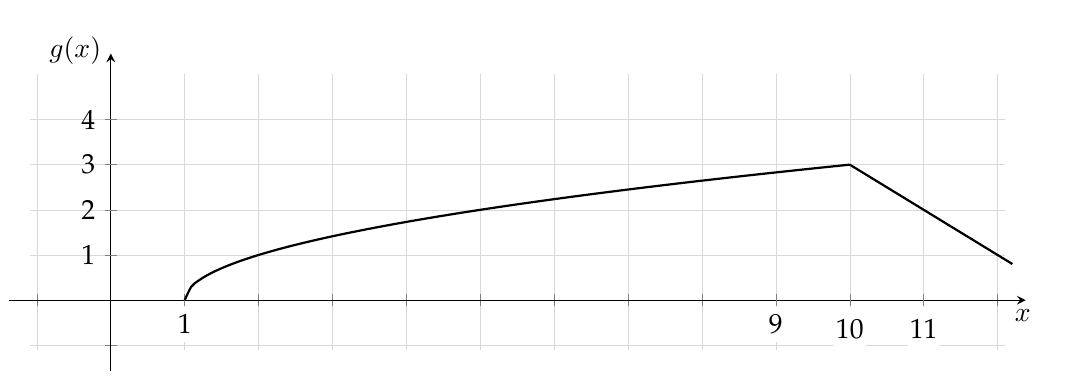
\begin{tikzpicture}[domain=-1:11] 
        \begin{axis}[
        width=5.5in,
        height=2in,
        grid=both,
        grid style={line width=.2pt, draw=gray!30},
        clip=false,
        axis lines=middle,
        xmin=-1.1,xmax=12.1,
        ymin=-1.1,ymax=5,
        restrict y to domain=-1:4,
        xtick={-2,-1,0,1,...,9,10,11,12},
        xticklabels={, , , , , , , , , ,},
        ytick={-1,0,1,2,3,4},
        yticklabels={, , , , , , , , , ,},
        extra x ticks={1,9,10,11},
        extra y ticks={1,2,3,4},
        extra x tick style={xticklabel style={fill=white, circle, inner sep=1.5pt}},
        extra y tick style={xticklabel style={fill=white, circle, inner sep=1.5pt}},
        extra x tick labels={1,9,10,11},
        extra y tick labels={1,2,3,4},
        axis line style={shorten >=-7.5pt, shorten <=-7.5pt},
        xlabel=$x$,
        ylabel=$g(x)$,
        xlabel style={at={(ticklabel* cs:1)},anchor=north west},
        ylabel style={at={(ticklabel* cs:1)},anchor=south east}
        ]
        \addplot[samples=100,domain=1:10,smooth, thick] {sqrt(x-1)} node[pos=1] (endofplotsquare) {};  
        \addplot[samples=100,domain=10:12.2,smooth, thick] {13-x} node[pos=1] (endofplotsquare) {};  
        \end{axis}
    \end{tikzpicture} 
    \end{center}
    
    \item Evaluate the following limits.
    \begin{enumerate}
    	\item \begin{align*} 
        \lim_{x \rightarrow 0^-} \frac 1 x - \frac{1}{|x|} 
        &= \lim_{x \rightarrow 0^-} \frac 1 x + \frac{1}{x} = -\infty
        \end{align*}
        This one-sided limit does not exist (DNE). 
    	\item Apply the sandwich (or squeeze) theorem. 
        \begin{align*} 
        	-x^2 \le x^2\sin\left(\frac{1}{x^4}\right) \le x^2\\
        	\lim_{x \rightarrow 0} -x^2 = \lim_{x \rightarrow 0} +x^2 = 0 \\
        	\Rightarrow \lim_{x \rightarrow 0} x^2\sin\left(\frac{1}{x^4}\right) = 0
        \end{align*}
    	\item 
        \begin{align*} 
         	\lim_{x \rightarrow 2} \frac{\frac 1 x - \frac 1 2}{x^2 - 4} 
            & =\lim_{x \rightarrow 2} \frac{\frac {2}{2x} - \frac {x}{2x}}{(x-2)(x+2)} \\
            & =\lim_{x \rightarrow 2} \frac {1}{2x} \frac{2 - x}{(x-2)(x+2)} \\
            & =\lim_{x \rightarrow 2} \frac {1}{2x} \frac{-(x-2)}{(x-2)(x+2)} \\
            & =\lim_{x \rightarrow 2} \frac{-1}{2x(x+2)} \\
            &= \frac{-1}{16}
		\end{align*}
    \end{enumerate}    
    
\end{enumerate}






%\newpage\section*{Worksheet 4, \Course, \Semester} 
\noindent \Sections 2.1, 2.6

\subsection*{Exercises}

\begin{enumerate}

    \item \TorF
    \begin{enumerate}
        \item If $y(t) \rightarrow 1$ as $t \rightarrow \infty$, then $y$ has the horizontal asymptote $y = 1$, and $y(t)$ is never equal to 1.      
    	\item {\large If $\displaystyle{\lim_{t\rightarrow 2}} \ t^2 \, f(t) = \infty$, then $\displaystyle{\lim_{t\rightarrow 2}} \, f(t) = \infty$ } 
        \item {\large $\displaystyle{\lim_{t\rightarrow \infty}} \left( t - \sqrt{t^2+16}\right) = \displaystyle{\lim_{t\rightarrow \infty}} \left( t - \left( \sqrt{t^2} + \sqrt{16}\right)\right) $ }
        \item {\large $\displaystyle{\lim_{t\rightarrow \infty}} \left( t - \sqrt{t^2+16}\right) = \infty - \infty = 0 $ }        
    \end{enumerate}
    
    \item If possible, sketch the graph of a function that satisfies the following criteria. If it is not possible to do so, state why. It isn't necessary to give a formula for the functions. 
	\begin{enumerate}
    	\item $f(x)$ is continuous, odd, $f(2) < -1$, $\displaystyle{\lim_{x\rightarrow\infty} f(x) = -1}$
    	\item $g(x)$ is continuous, even, $\displaystyle{\lim_{x\rightarrow-\infty} g(x) = -2}$, and $\displaystyle{\lim_{x\rightarrow \infty} g(x) =2}$        
    \end{enumerate}
	\item If possible, evaluate the following limits. If they do not exist, state why.

	\begin{enumerate}\setlength\itemsep{12pt}
    
		\item $\displaystyle{\lim_{x\to 5^-} \left(\frac{3x}{2x-10}\right)}$

		\item $\displaystyle{\lim_{t\to \infty}\ln\left(1+\frac{1}{t}\right)}$
    
		\item $\displaystyle{\lim_{x\to \infty} \left(\frac{2+\sqrt{x}}{2-\sqrt{x}}\right)}$

\end{enumerate}

	\item Identify all asymptotes (horizontal, vertical, oblique) of the function $f(x) = \displaystyle {\frac{x^3-4x^2+3x}{3x^2-6x}}$

	\item The position of an object is given by $y(t) = t^2 + 2t$. 
    \begin{enumerate}
    	\item Give an expression for the average speed of the object over the interval $[1,1+\Delta t]$, where $\Delta t > 0$. 
        \item Use your expression in part (a) to calculate the average speed of the object over the interval $[1,2]$. 
        \item Use your expression in part (a) to calculate the instantaneous speed when $t = 1$. 
    \end{enumerate}
\end{enumerate}    
%\newpage\subsection*{1551 Worksheet 4 Answers}

\SolutionsStatement

\begin{enumerate}
    
    \item \begin{enumerate} 
    	\item False. The graph of a function can cross a horizontal asymptote. For example: $1+\sin(t)/t$. 
    	\item True. The limit of the product is the product of the limits:
        \begin{align*}
        	\lim_{t\rightarrow 2} \ t^2 \, f(t) &= \infty\\
            \lim_{t\rightarrow 2} \ t^2 \, \lim_{t\rightarrow 2} f(t) &= \infty\\
            4 \, \lim_{t\rightarrow 2} f(t) &= \infty\\
            \lim_{t\rightarrow 2} f(t) &= \infty
        \end{align*}
        \item False. Because $\sqrt{a+b} \ne \sqrt{a} + \sqrt{b}$ for all $a$ and $b$.
        \item False. Because $\infty - \infty$ is undefined. 
    \end{enumerate}
    The limit in parts (c) and (d) is explored in our textbook, \Textbook. See Example 9, Section 2.6, page 108. 
    
    \item \begin{enumerate}
    	\item Possible, see graph below. 
		\begin{center}
			\includegraphics[width=0.8\textwidth]{images/imgWS4Spring17.png} 
		\end{center}
    
        \item Impossible. If $g$ is even, then $g$ is symmetric about the line $x=0$, so 
        $$\lim_{x\rightarrow\infty} g(x) = \lim_{x\rightarrow-\infty} g(x)$$
    \end{enumerate}    
    
    \item \begin{enumerate}\setlength\itemsep{12pt}
    
		\item $\displaystyle{\lim_{x\to 5^-} \left(\frac{3x}{2x-10}\right)} = -\infty$

		\item $\displaystyle{\lim_{t\to \infty}\ln\left(1+\frac{1}{t}\right)}
 = \ln(1 + 0) = \ln(1) = 0 $
 
		\item \begin{align*} 
        	\lim_{x\to \infty} \left(\frac{2+\sqrt{x}}{2-\sqrt{x}}\right) &= 
        	\lim_{x\to \infty} \left(\frac{2+\sqrt{x}}{2-\sqrt{x}}\right)\left(\frac{2-\sqrt{x}}{2-\sqrt{x}}\right) \\ &=
            \lim_{x\to \infty} \left(\frac{4-x}{4-2\sqrt{x}+x}\right)  \\ &= 
            \lim_{x\to \infty} \left(\frac{4/x-1}{4/x-\frac{2}{\sqrt{x}}+1}\right)  \\ &= 
            \frac{-1}{1} \\ &= 
            -1
            \end{align*}

	\end{enumerate}

	\item Horizontal asymptotes: 
    \begin{align*} 
    	\lim_{x\to \pm \infty } \left(\frac{x^3-4x^2+3x}{3x^2-6x}\right) = \pm \infty 
    \end{align*}
    Therefore no horizontal asymptotes. Vertical asymptotes: 
	\begin{align*} 
    	\frac{x^3-4x^2+3x}{3x^2-6x} &= \frac{x^2-4x+3}{3x-6}\\
        &= \frac{(x-1)(x-3)}{3x-6}\\
    	\lim_{x\to 2 ^- } \frac{(x-1)(x-3)}{3x-6} &= +\infty \\
    	\lim_{x\to 2 ^+ } \frac{(x-1)(x-3)}{3x-6} &= -\infty 
    \end{align*}
	For the oblique asymptotes, use polynomial division to obtain:
    \begin{align*} 
    	f(x) &= \frac{x^2-4x+3}{3x-6} = \frac x 3 - \frac 2 3 - \frac{1}{3x - 6}
    \end{align*}
	Thus, $f$ has the oblique asymptote $\frac x 3 - \frac 2 3$.
    
    \item 
    \begin{enumerate}
    	\item \begin{align*}
        \text{average speed at time } t \text{ over interval } [t,t+\Delta t]&= \frac{(t+\Delta t)^2 + 2(t+\Delta t) - (t^2 + 2t)}{\Delta t} \\
        &= \frac{ (\Delta t)^2 + 2 \Delta t\, t + 2 \Delta t}{\Delta t} \\
        &= \Delta t + 2t + 2 \\
		\text{average speed at time } 1 \text{over interval } [1,1+\Delta t]
        &= \Delta t + 2(1) + 2 \\ 
        &= \Delta t + 4
        \end{align*}
        \item $\Delta t = 1$, so average speed over $[1,2]$ is $\Delta t+4 = 5$. 
        \item instantaneous speed at $t = 1$ is $$\lim_{\Delta t \rightarrow 0} (\Delta t + 2t + 2 )\huge|_{t = 1} =  (0+2t + 2) \huge|_{t = 1} = 4$$
    \end{enumerate}
\end{enumerate}






%\newpage\section*{Worksheet 5, \Course, \Semester} 
\noindent \Sections 3.1, 3.2, 3.3

\subsection*{Exercises}

\begin{enumerate}

    \item This question explores some of the questions on Midterm 1.     
    \begin{enumerate}
        \item \TorFShort \\If $\displaystyle{\lim_{x\rightarrow a} f(x) =L}$, then $f(a) = L$.   		\item If possible, construct the inverse function $f^{-1}$ of $f(x) = x^2 -4x$ over the domain $x \in [4,6]$.
    \end{enumerate}
    \item Let $f(x)=\sqrt{5-x}$.
	\begin{enumerate}
		\item Use the limit definition of the derivative to compute the derivative of the function.
		\item For what values of $x$ is $f$ differentiable? Write your answer as an interval. 
	\end{enumerate}
    \item Identify all points $(x,y)$ on the graph of
  $$g(x)=\frac{1}{3}x^3-\frac{3}{2}x^2+1$$ where the tangent line is parallel to the line $8x-2y=1$.

	\item Sketch a function, $y(x)$, that is defined on the domain $x\in[-4,4]$, is continuous, odd, and not differentiable at exactly two points. Label your axes. 
    \item Give a formula for a function $y(x)$, that is continuous everywhere but not differentiable at $x = 1$.
    \item Compute the slope of the tangent line to $f(x)$ at the point where $x = 1$.
    
    $$f(x) = \frac{5x + 1}{4x^2 + 1}$$
\end{enumerate}    
%\newpage\subsection*{1551 Worksheet 5 Answers}

\SolutionsStatement

\begin{enumerate}
    
    \item See midterm 1 solutions. 
	\item \begin{enumerate}
    \item \begin{align*} 
    	f'(x) &= \lim_{h\to 0}\frac{f(x+h)-f(x)}{h} \\
        &= \lim_{h\to 0} \frac 1 h \left( \sqrt{5 - x - h} - \sqrt{5-x} \right) \\
        &= \lim_{h\to 0} \frac 1 h \left( \sqrt{5 - x - h} - \sqrt{5-x} \right)\left( \frac{\sqrt{5 - x - h} + \sqrt{5-x}}{ \sqrt{5 - x - h} + \sqrt{5-x} } \right) \\
        &= \lim_{h\to 0} \frac 1 h \left( \frac{(5 - x - h) - (5-x)}{ \sqrt{5 - x - h} + \sqrt{5-x} } \right) \\
        &= \lim_{h\to 0} \left( \frac{-1}{ \sqrt{5 - x - h} + \sqrt{5-x} } \right) \\
        &=  \frac{-1}{ 2\sqrt{5-x} }
    \end{align*}
    
    \item $(-\infty,5]$    
\end{enumerate}
	\item We want points on the curve where $g'(x)$ is equal to the slope of the line $8x - 2y = 1 $.
    \begin{align*}
    	8x - 2y &= 1 \\
        2y &= 8x - 1 \\
        y &= 4x - 1/4
    \end{align*}
    So the slope of the line is 4. 
    \begin{align*}
    	4 &= g'(x) \\
        4 &= \ddx \left(\frac{1}{3}x^3-\frac{3}{2}x^2+1 \right)\\
        4 &= x^2 -3x + 0 \\ 
        0 &= x^2 -3x -4 \\
        0 &= (x+1)(x-4)
    \end{align*}    
    At $x=-1$ and $x=4$ the tangent line has the desired slope. Evaluating $g(x)$ at these points yields the points $(-1,-5/6)$, and $(4,-5/3)$. 
    \newpage 
    
    \item There are many acceptable solutions. But note that for the function to be odd and continuous, it must pass through the origin. 
    
    	\begin{center}
		\includegraphics[width=0.85\textwidth]{images/imgWS5OddSpring17.png} 
	\end{center}
    
    \item Many acceptable solutions, including $y(x) = |x-1|$.
    \item \begin{align*}
    f'(x) 
    &= \ddx \ \frac{5x + 1}{4x^2 + 1} \\
    &= \frac{\ddx (5x+1) (5x^2 + 1) - (5x+1)\ddx(4x^2+1)}{(4x^2+1)^2} \\
    &= \frac{5 (5x^2 + 1) - (5x+1)(8x)}{(4x^2+1)^2} \\
    f'(1) &= \frac{5\cdot 6 - 6\cdot 8}{5^2} \\
    &= \frac{30 - 48}{25} \\
    &= -\frac{18}{25}
   \end{align*}
\end{enumerate}






%\newpage\section*{Worksheet 6, \Course, \Semester} 
\noindent \Sections 3.4, 3.5, 3.6

\subsection*{Exercises}

\begin{enumerate}
    
    \item A moving object has positive velocity for times $t \in [0,2)$, negative velocity for $t \in (2,4]$, and negative acceleration for $t\in[0,4]$. 
    \begin{enumerate}
        \item Sketch a graph that could represent the objects' position for $t \in [0,4]$. Label your axes.  
        \item Give a formula that could represent the objects' position for $t \in [0,4]$.
    \end{enumerate}
    \item The graph below gives the position of a moving object, $s(t)$ as a function of time, $t$. \begin{enumerate} \item Sketch the velocity and the speed of the object on two separate graphs. \item When the speed constant? \item When is the acceleration non-zero? \end{enumerate}
        \begin{center}
    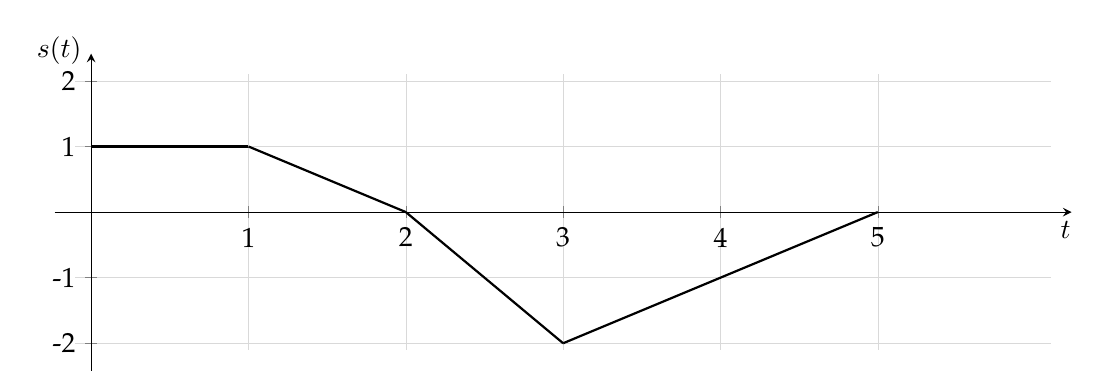
\begin{tikzpicture}[domain=0:6] 
        \begin{axis}[
        width=5.5in,
        height=2in,
        grid=both,
        grid style={line width=.2pt, draw=gray!30},
        clip=false,
        axis lines=middle,
        xmin=-0.1,xmax=6.1,
        ymin=-2.1,ymax=2.1,
        xtick={0,1,2,3,4,5},
        xticklabels={0,1,2,3,4,5},
        ytick={-2,-1,0,1,2},
        yticklabels={-2,-1,0,1,2},
        axis line style={shorten >=-7.5pt, shorten <=-7.5pt},
        xlabel=$t$,
        ylabel=$s(t)$,
        xlabel style={at={(ticklabel* cs:1)},anchor=north west},
        ylabel style={at={(ticklabel* cs:1)},anchor=south east}
        ]
        \addplot[samples=100,domain=0:1,smooth, thick] {1} node[pos=1] (endofplotsquare) {};
        \addplot[samples=100,domain=1:2,smooth, thick] {2-x} node[pos=1] (endofplotsquare) {};
        \addplot[samples=100,domain=2:3,smooth, thick] {4-2*x} node[pos=1] (endofplotsquare) {};        
        \addplot[samples=100,domain=3:5,smooth, thick] {x-5} node[pos=1] (endofplotsquare) {};        
        \end{axis}
    \end{tikzpicture}   
    \end{center}    

    \item \TorF
    \begin{enumerate}
    	\item If $f(x)$ and $g(x)$ are differentiable on the interval $(a,b)$, and $f(x) > g(x)$ over $(a,b)$, then $f'(x) > g'(x)$ on the interval $(a,b)$. 
        \item If $f(x)$ is differentiable for all $x$, and $f(0) = f'(0) = 0$, then $f(x) = 0$ for all $x$. 
        \item If the position of a moving object, $s(t)$, is differentiable for $t\in[0,1]$, and the velocity of the object is positive over $t \in [0,1]$, then the acceleration must also be positive over $t\in[0,1]$. 
    \end{enumerate}    
    
    \item Construct an equation of the tangent line to $y(x)$ at $x= 0$. $$y(x) = \frac{2e^x}{x^2-1}$$
    
	\item Differentiate the following functions. 
    
    \begin{enumerate}
    	\item $y = 1 + f(x^2) g(h(x))$
        \item $y = \frac{3+9\tan x}{\sec x}$
    \end{enumerate}
    
\end{enumerate}
%\newpage\subsection*{1551 Worksheet 6 Answers}

\SolutionsStatement

\begin{enumerate}
    
    \item \begin{enumerate}
    
    	\item A solution is shown below. Many acceptable answers.
        
        \begin{center}
    	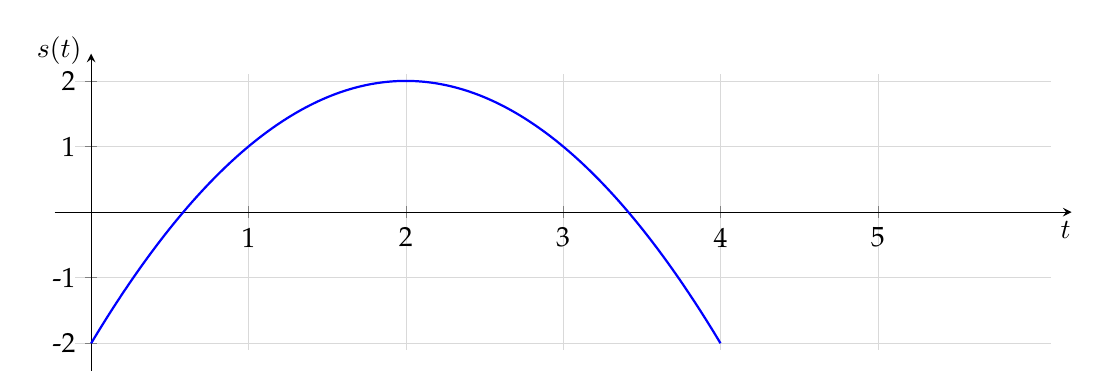
\begin{tikzpicture}[domain=0:6] 
        \begin{axis}[
        width=5.5in,
        height=2in,
        grid=both,
        grid style={line width=.2pt, draw=gray!30},
        clip=false,
        axis lines=middle,
        xmin=-0.1,xmax=6.1,
        ymin=-2.1,ymax=2.1,
        xtick={0,1,2,3,4,5},
        xticklabels={0,1,2,3,4,5},
        ytick={-2,-1,0,1,2},
        yticklabels={-2,-1,0,1,2},
        axis line style={shorten >=-7.5pt, shorten <=-7.5pt},
        xlabel=$t$,
        ylabel=$s(t)$,
        xlabel style={at={(ticklabel* cs:1)},anchor=north west},
        ylabel style={at={(ticklabel* cs:1)},anchor=south east}
        ]
        \addplot[samples=100,domain=0:4,smooth, thick, blue] {2 - (x-2)*(x-2)} node[pos=1] (endofplotsquare) {}; 
        \end{axis}
    \end{tikzpicture}   
    \end{center}    
        
        \item Many acceptable answers, including $s(t) = 2 - (t - 2)^2$. 
    
	\end{enumerate}
    
    \item \begin{enumerate}
    
    	\item The velocity and speed are shown below. 
        \begin{center}
    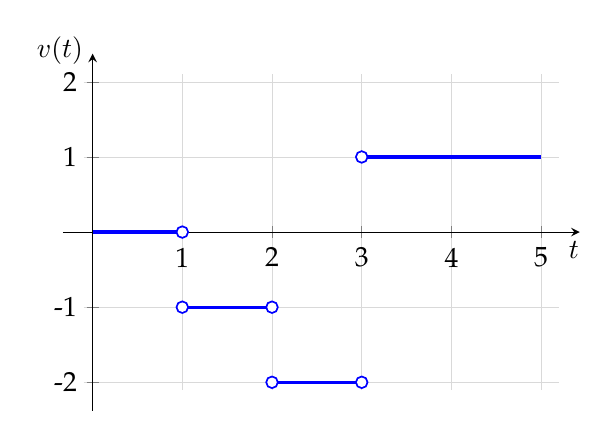
\begin{tikzpicture}[domain=0:5.2] 
        \begin{axis}[
        width=3in,
        height=2.2in,
        grid=both,
        grid style={line width=.2pt, draw=gray!30},
        clip=false,
        axis lines=middle,
        xmin=-0.1,xmax=5.2,
        ymin=-2.1,ymax=2.1,
        xtick={0,1,2,3,4,5},
        xticklabels={0,1,2,3,4,5},
        ytick={-2,-1,0,1,2},
        yticklabels={-2,-1,0,1,2},
        axis line style={shorten >=-7.5pt, shorten <=-7.5pt},
        xlabel=$t$,
        ylabel=$v(t)$,
        xlabel style={at={(ticklabel* cs:1)},anchor=north west},
        ylabel style={at={(ticklabel* cs:1)},anchor=south east}
        ]
        \addplot[samples=100,domain=0:1,smooth, very thick, blue] {0} node[pos=1] (endofplotsquare) {};
        \addplot[samples=100,domain=1:2,smooth, very thick, blue] {-1} node[pos=1] (endofplotsquare) {};
        \addplot[samples=100,domain=2:3,smooth, very thick, blue] {-2} node[pos=1] (endofplotsquare) {};        
        \addplot[samples=100,domain=3:5,smooth, very thick, blue] {1} node[pos=1] (endofplotsquare) {};        
        \addplot[blue,mark=o,thick] coordinates {(1,+0)};
        \addplot[blue,mark=o,thick] coordinates {(1,-1)};
        \addplot[blue,mark=o,thick] coordinates {(2,-1)};
        \addplot[blue,mark=o,thick] coordinates {(2,-2)};
        \addplot[blue,mark=o,thick] coordinates {(3,-2)};
        \addplot[blue,mark=o,thick] coordinates {(3,+1)};        
        \addplot[white,mark=*, mark size=1.5] coordinates {(1,+0)};
        \addplot[white,mark=*, mark size=1.5] coordinates {(1,-1)};
        \addplot[white,mark=*, mark size=1.5] coordinates {(2,-1)};
        \addplot[white,mark=*, mark size=1.5] coordinates {(2,-2)};
        \addplot[white,mark=*, mark size=1.5] coordinates {(3,-2)};
        \addplot[white,mark=*, mark size=1.5] coordinates {(3,+1)};
        \end{axis}
    \end{tikzpicture}   
    \end{center}    
    \vspace{12pt}
    \begin{center}
    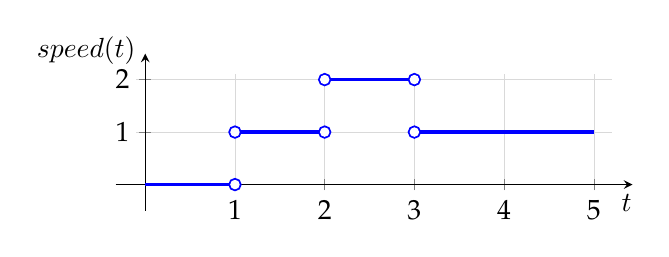
\begin{tikzpicture}[domain=0:5.2] 
        \begin{axis}[
        width=3in,
        height=1.2in,
        grid=both,
        grid style={line width=.2pt, draw=gray!30},
        clip=false,
        axis lines=middle,
        xmin=-0.1,xmax=5.2,
        ymin=-0.1,ymax=2.1,
        xtick={0,1,2,3,4,5},
        xticklabels={0,1,2,3,4,5},
        ytick={-2,-1,0,1,2},
        yticklabels={-2,-1,0,1,2},
        axis line style={shorten >=-7.5pt, shorten <=-7.5pt},
        xlabel=$t$,
        ylabel=$speed(t)$,
        xlabel style={at={(ticklabel* cs:1)},anchor=north west},
        ylabel style={at={(ticklabel* cs:1)},anchor=south east}
        ]
        \addplot[samples=100,domain=0:1,smooth, very thick, blue] {0} node[pos=1] (endofplotsquare) {};
        \addplot[samples=100,domain=1:2,smooth, very thick, blue] {1} node[pos=1] (endofplotsquare) {};
        \addplot[samples=100,domain=2:3,smooth, very thick, blue] {2} node[pos=1] (endofplotsquare) {};        
        \addplot[samples=100,domain=3:5,smooth, very thick, blue] {1} node[pos=1] (endofplotsquare) {};        
        \addplot[blue,mark=o,thick] coordinates {(1,0)};
        \addplot[blue,mark=o,thick] coordinates {(1,1)};
        \addplot[blue,mark=o,thick] coordinates {(2,1)};
        \addplot[blue,mark=o,thick] coordinates {(2,2)};
        \addplot[blue,mark=o,thick] coordinates {(3,2)};
        \addplot[blue,mark=o,thick] coordinates {(3,1)};        
        \addplot[white,mark=*, mark size=1.5] coordinates {(1,0)};
        \addplot[white,mark=*, mark size=1.5] coordinates {(1,1)};
        \addplot[white,mark=*, mark size=1.5] coordinates {(2,1)};
        \addplot[white,mark=*, mark size=1.5] coordinates {(2,2)};
        \addplot[white,mark=*, mark size=1.5] coordinates {(3,2)};
        \addplot[white,mark=*, mark size=1.5] coordinates {(3,1)};
        \end{axis}
    \end{tikzpicture}   
    \end{center}    
        
        \item Speed is constant over $[0,1)\cup(1,2)\cup(2,3)\cup(3,5]$. At $t=0$ and $t = 5$, we are using the concept of differentiability on an interval, from Section 3.2. For more details see textbook, page 130. Or see lecture slides for section 3.2, slide 5. Or see lecture slides for section 3.4, slide 10. 
        
        \item Velocity is undefined at times $t = 1,2,3$. 
        
        \item Acceleration, wherever it is defined, is always zero because the velocity is piecewise constant. 
    
	\end{enumerate}
    
    \item \begin{enumerate}
    
    	\item False. Counterexample: $f = x + 10$, $g = 2x$ over $x\in(0,1)$.
    
        \item False. Counterexample: $f = x^2$.
        
        \item False. Counterexample: $f = \sin(t)$. Another counterexample is $f=2 - (t-1)^2$, which is the same function in question 1b.
    
	\end{enumerate}
    
    \item \begin{align*}
    	y'(x) &= \ddx \frac{2e^x}{x^2-1} \\
        &= \ddx 2e^x(x^2-1)^{-1} \\
        &= 2e^x (x^2 -1)^{-1} - 2e^x (x^2 - 1)^{-2}(2x) \\
        y'(0) &= 2e^0 (0^2 -1)^{-1} - 2e^0 (0^2 - 1)^{-2}(2\cdot 0) = -2 \\
        y(0) &= \frac{2e^x}{x^2-1} = -2 \\
        y - y(0) &= y'(0)(x-x_0) \\
        y - (-2) &= -2(x-0) \\    
        y &= -2x -2
    \end{align*}
    
    
    \begin{enumerate}
    	\item $y = 1 + f(x^2) g(h(x))$: 
        \begin{align*}
        	y' 
            &= 0 + \ddx  f(x^2) g(h(x)) \\
            &= 2xf'(x^2) g(h) + f(x^2)g'(h)h'
        \end{align*}
        \item $y = \frac{3+9\tan x}{\sec x}$:
        \begin{align*}
        	y' 
            &= \ddx \frac{3+9\tan x}{\sec x} \\
            &= \ddx \left(\frac{3}{\sec x} + \frac{9\tan x}{\sec x} \right)\\
            &= \ddx \left( 3\cos x + 9\sin x \right)\\
            &= -3\sin x + 9\cos x 
        \end{align*}        
    \end{enumerate}    
\end{enumerate}

%\newpage\section*{Worksheet 7, \Course, \Semester} 
\noindent \Sections 3.7, 3.8, 3.9

\subsection*{Exercises}

\begin{enumerate}
	\item Differentiate the following functions. 
    \begin{enumerate}
    	\item $\displaystyle v(t) = 2^{3t}$
    	\item $\displaystyle y(x) = {\large x^{x^{x}}}, \quad x > 0$
        \item $\displaystyle u(x) = \sin\left(\tan^{-1} (\ln x)\right)$
        
        \item $\displaystyle s(t) = \log_2\left(\log_3\left(e^{t^2}\right)\right)$
        \item $\displaystyle a(t) = \ln\left(\frac{(t+2)^3(t+5)^7}{\sqrt{t-5}}\right)$
    \end{enumerate}
    \item The curve below is specified by the equation $$2\left(x^2+y^2\right)^2=25\left(x^2-y^2\right)$$
    
    \begin{center}
		\includegraphics[width=0.7\textwidth]{images/imgWS7Implicit.png} 
    \end{center}
    
    
    
    
    \begin{enumerate}
    	\item By inspection, is the slope of the tangent line at $(3,1)$ positive, negative, or zero? 
        \item Construct the equations of the tangent line, and the normal line, at the point $(3,1)$. 
\end{enumerate}
\end{enumerate}
%\newpage\subsection*{1551 Worksheet 7 Answers}

\SolutionsStatement

\begin{enumerate}
    
    \item \begin{enumerate}
    
    \item \begin{align*}
    	v'(t) &= \ddt 2^{3t} 
        = 2^{3t} \ln 2 \ddt (3t)  
        = 3\cdot 2^{3t} \ln 2
    \end{align*}
    Alternate solution: 
    \begin{align*}
    	v'(t) &= \ddt 2^{3t}
        = \ddt 8^t 
        = 8^t \ln 8
    \end{align*}
    
    	\item 
    	\begin{align*} 
    		y(x) &= x^{x^{x}} \\
    		\ln y&= \ln x^{x^{x}} =x^x \ln x \\
     		\frac{y'}{y} &= \ddx (x^x \ln x) \\
     		&= ( \ddx x^x ) \ln x + x^x \ddx \ln x \\
     		&= ( \ddx x^x ) \ln x + x^x \frac 1 x 
    	\end{align*}
    	Calculate the derivative of $x^x$: 
        \begin{align*}
        	\text{let } u = x^x, \text{then } \ln u &= x \ln x \\
            \frac{u'}{u} &= \ddx ( x \ln x) = \ln x + 1 \\
            u' &= u(\ln x + 1) 
            = x^x (\ln x + 1) 
        \end{align*}
        Thus $y'= x^x (\ln x + 1) \ln x + x^{x-1}$. 

        
        
        \item \begin{align*} 
        	u(x) &= \sin\left(\tan^{-1} (\ln x)\right) \\
            \ddx u 
            &= \cos\left(\tan^{-1} (\ln x)\right) \cdot 
            \ddx \left(\tan^{-1} (\ln x)\right) \\
            &= \cos\left(\tan^{-1} (\ln x)\right) \cdot 
            \frac{1}{1+ (\ln x)^2} \cdot \ddx \ln x \\    
            &= \cos\left(\tan^{-1} (\ln x)\right) \cdot 
            \frac{1}{1+ (\ln x)^2} \cdot \frac 1 x            
        \end{align*}
        
        
        
        
        \item \begin{align*} 
        	s(t) &= \log_2\left(\log_3\left(e^{t^2}\right)\right) \\
            s' 
            &= \frac{1}{\log_3\left(e^{t^2}\right) \ln 2} \cdot \ddt  \left( \log_3 e^{t^2} \right) \\
            &= \frac{1}{\log_3\left(e^{t^2}\right) \ln 2} \cdot  \frac{1}{ \log_3 e^{t^2}} \cdot \ddt e^{t^2} \\
            &= \frac{1}{\log_3\left(e^{t^2}\right) \ln 2} \cdot  \frac{1}{ \log_3 e^{t^2}} \cdot e^{t^2} \cdot 2t           
        \end{align*}
        
        
        \item \begin{align*}
        a(t) 
        &= \ln\left(\frac{(t+2)^3(t+5)^7}{\sqrt{t-5}}\right) \\
        &= 3 \ln\left(t+2 \right) + 7 \ln\left(t+5\right) - \frac 1 2 \ln \left( t-5\right) \\
        a'(t) &= \frac{3}{t+2} +\frac{7}{t+5} - \frac{1}{2(t-5)} 
        \end{align*}
    \end{enumerate}
    
    
    
    
    
    
    
    \item \begin{enumerate}
    	\item Negative. Because if the tangent line is $y=mx +b$, value of $y$ decreases as $x$ increases.
        \item Use implicit differentiation. Assume $y=y(x)$. 
        \begin{align*}
        	\ddx 2\left(x^2+y^2\right)^2&= \ddx 25\left(x^2-y^2\right) \\
        	4(x^2+y^2) \cdot (2x+ 2y y') &= 25(2x-2yy') 
        \end{align*}
        Now substitute $(3,1)$ and solve for $y'$. 
        \begin{align*}        
        	4(3^2+1^2) \cdot (2\cdot3+ 2 y') &= 25(2\cdot3-2\cdot1\cdot y')\\
        	40 (6+ 2 y') &= 25(6 - 2y')\\
             (6+ 2 y') &= \frac 5 8 (6 - 2y')\\
            \frac 13 4 y' &= - \frac 9 4 \\
            y' &= - 9 13
        \end{align*}
        Thus the equation of the tangent line is 
        \begin{align*}
        	y - 1 &= - \frac{9 }{13} (x - 3) \\
            y &= 1 - \frac{9}{ 13} (x - 3)
        \end{align*}
        The slope of the line is negative, as expected. The equation of the normal line is
        \begin{align*}
            y &= 1 + \frac{13}{ 9} (x - 3)
        \end{align*}       
    \end{enumerate}

    
\end{enumerate}    








%\newpage\section*{Worksheet 8, \Course, \Semester} 
\noindent \Sections 3.10, 3.11

\subsection*{Related Rate Problems}

    Solving rate problems tend to involve the following sequence of steps.
    \begin{enumerate}
        \item Read the question.
        \item Draw a diagram.
        \item Introduce variables.
        \item Construct an equation.
        \item Calculate derivative at a point.
        \item Express answer to question using appropriate units. 
    \end{enumerate}
    Please express your final answer with units. 
    
    
\subsection*{Exercises}

\begin{enumerate}
	\item Construct the linearization of $f(x) = \ln(x-1)$ centered at $x=2$ and use it to approximate the value of $f(3)$. Plot your linearization and $f(x)$ on the same graph.
    
	\item An 5ft ladder is leaning against a vertical wall. If the bottom of the ladder is pulled away from the wall at a constant rate of 3 ft/sec, calculate the rate at which the top is sliding down the wall when the bottom is 4ft from the wall. 

	\item The diameter and height of a right circular cylinder are found at a certain instant to be 10cm and 20cm, respectively. If the diameter is increasing at the rate of 1cm/sec, what change in height will keep the volume constant?

	\item A cubical magnet is measured to have side lengths of 4cm within an error range of 0.3cm. Use differentials to find the maximum error in measuring the volume of the magnet. 

	\item A particle moves in a circular orbit $x^2+y^2=1$. As it passes through the point $\left(\frac{1}{2},\frac{\sqrt{3}}{2}\right)$, its $y$-coordinate decreases at the rate of 3 units/sec. At what rate is the $x$-coordinate changing? 

\end{enumerate}
%\newpage\subsection*{1551 Worksheet 8 Answers}
\begin{enumerate}
    
    \item \begin{align*}
     f(x) &= \ln(x-1) \\
     f'(x) &= \frac{1}{x-1} \\
     f'(2) &= 1   
     \end{align*}
	The linearization $L(x)$ near $x = 2$ is
    \begin{align*}
     L(x) &= f(2) + f'(2)(x - 2) \\
     &= ln(1) + (x - 2) \\
     &= x - 2
    \end{align*}
    At $x=3$, $f(3) \approx L(3) = 3 - 1 = 2$. 
    
	\begin{center}
		\includegraphics[width=0.8\textwidth]{images/imgWS8ln.png} 
	\end{center}    
    
    
    \item Let $x=x(t)$ be the horizontal distance from wall, $y=y(t)$ is the vertical distance between floor and the top of the ladder. Using the Pythagorean Theorem, when $x$ = 8, $$y = \sqrt{5^2 -4^2} = 3$$
    The Pythagorean Theorem and differentiation gives us
    \begin{align*}
    	5^2 &= x^2 + y^2 \\
        \ddt 18^2 &= \ddt (x^2 + y^2) \\
        0 &= 2x \dxdt + 2y \dydt \\
        0 &= 2\cdot 8 \cdot 3 + 2\cdot 3 \dydt \\
        \dydt &= -8 
    \end{align*}
	The top of the ladder is falling at a rate of 8 ft/s (we could also write this as `the height of the ladder is changing at a rate of -8 ft/s'). \\[12pt] \textit{For full marks, state answer with units}.
    
   \item Use $V = \pi r^2 h$ and differentiate.
   \begin{align*}
   	V &= \pi r^2 h \\
    \ddt V &= \ddt (\pi r^2 h )\\
    V' 
    &= \pi (2rr'h + r^2h')  \\
    &= \pi (2\cdot 5 \cdot r' \cdot 20 + (5)^2h') \\
    &= \pi (200 r'  + 25h') \\
   \end{align*}
   If $D$ is the diameter, and $\frac{dD}{dt} = 1$, then 
   \begin{align*}
   		D&= 2r \\
        \frac{dD}{dt} &= 2 \frac{dr}{dt} \\
        1 &=2 r' \\
        r' &= \frac 1 2
   \end{align*}
   Set $V' = 0$, and solve for $h'(t)$. 
   \begin{align*}
    	0 &= \pi (200 r'  + 25h') \\
    	0 &= \pi (200 \cdot \frac 1 2  + 25h') \\
        h' &= -4
   \end{align*}   
   The height must decrease at a rate of 4 cm/s. 
   
   \item Let $x$ be the side length of the magnet. 
   \begin{align*}
   	\text{volume} = V &= x^3 \\
    dV &= v'(r) \, dr \\
    &= 3r^2 dr \\
    &= 3 \cdot (4)^2 \cdot 0.3 \\
    &= \frac{144}{10} \ \text{cm}^3
   \end{align*}
   The maximum error is 14.4 cm$^3$.
   
   \item 
   \begin{align*}
   		1 &= x^2 + y^2 \\
        0 &= 2x\dxdt + 2y\dydt \\
        \dxdt &= -\frac y x \dydt \\
        &= -\frac{\sqrt 3 /2 }{1/2} (-3) \\
        &=  3\sqrt 3
   \end{align*}
   The $x$-coordinate is changing at a rate of $3\sqrt 3$ units/second.
\end{enumerate}



















%\newpage\section*{Worksheet 9, \Course, \Semester} 
\noindent \Sections 4.1,4.2,4.3

\subsection*{A Few Definitions and Theorems from Sections 4.1, 4.2, 4.3}

	\begin{itemize}
    	\item \Emph{Local Extrema:} A function has a \Emph{local maximum} at $x = c$ if $f(x) \le f(c)$ for all $x$ in an open interval containing $c$. A function has a \Emph{local minimum} at $x = c$ if $f(x) \ge f(c)$ for all $x$ in an open interval containing $c$. 
        \item \Emph{Critical Points:} An interior point of the domain of $f(x)$ where $f'=0$, or where $f'$ is undefined, is a \Emph{critical point}. 
        \item \Emph{MVT:} If $f(x)$ is a continuous function defined on $[a,b]$, and is differentiable over $(a,b)$. Then there is at at least one point, $c \in (a,b)$, where 
        $$\frac{f(b)-f(a)}{b-a} = f'(c)$$ 
        \item \Emph{Increasing and Decreasing:} If $f'(x) > 0$ on $(a,b)$, then $f$ is \Emph{increasing} on $[a,b]$. If $f'(x) < 0$ on $(a,b)$, then $f$ is \Emph{decreasing} on $[a,b]$.
        \item \Emph{First Derivative Test:} Suppose $f$ has a critical point at $x=c$.
        \begin{itemize}
            \item If $f'(x)$ changes from positive to negative at $c$, then $f$ has a \Emph{local maximum} at $c$.
            \item If $f'(x)$ changes from negative to positive at $c$, then $f$ has a \Emph{local minimum} at $c$.
            \item If $f'(x)$ doesn't change sign from positive to negative at $c$, then $f$ has no local minimum or maximum at $c$.
        \end{itemize}
    \end{itemize}
    
\subsection*{Exercises}

\begin{enumerate}
	\item If possible, sketch a curve or give a formula for a function that has the following properties. If it is not possible to do so, state why. Assume in each case that $f(x)$ is continuous, differentiable, and defined for all values of $x$. 
    
    \begin{enumerate}
        \item $f(x)$ has a local maximum at $x=0$, and $f'(x)<0$ over the interval $(-1,1)$. 
        \item $f(x)$ has a local maxima at $x=0$ and $x=1$, $f(x)$ has no local minima. 
        \item $f(x)$ is odd, and has local maxima at $x=1$ and $x=2$.
    \end{enumerate}
    
	\item Which of the following functions satisfy the conditions of the 
Mean Value Theorem on the interval $[0,1]$? For those that do not, state why. For those that do, identify all values of $c$ so that $f'(c)=\frac{f(b)-f(a)}{b-a}$. 

	\begin{enumerate}
    	\item $\displaystyle f(x)=\sqrt{x(1-x)}$
        \item $\displaystyle f(x)=|x-0.5|$
    \end{enumerate}
    
	\item For each function below: (a) determine the interval(s) on which the 
function is increasing and/or decreasing; (b) Identify the local and 
absolute extreme values (if any) and where they occur. 
	\begin{enumerate} 
    	\item $\displaystyle f(x)=\frac{x^3}{3x^2+1}$
        \item $\displaystyle g(x)=x\ln x$
        \item $\displaystyle h(x)=x^{2/3}(x+5)$
    \end{enumerate} 



\end{enumerate}
%\newpage\subsection*{\Course Worksheet 9 Answers}
\begin{enumerate}
    
    \item 
    \begin{enumerate}
        \item Not possible: if there is a local max at $x=0$, then $f'$ has to change from negative to positive over interval $(-1,1)$, so $f'$ can't be negative over $(-1,1)$. 
        \item Not possible: if there is a local max at $x=0$ and $x=1$ and $f$ is continuous and differentiable everywhere, then there must be a local minimum between $x=0$ and $x=1$. 
    \end{enumerate}
    
    
    
    
    
    \item 
    \begin{enumerate}
        \item $f$ is continuous on $[0,1]$ and differentiable for $(0,1)$, so the function satisfies the conditions of the MVT. 
        \begin{align*}
        	f'(x) 
            &= \ddx (x(1-x))^{1/2}\\
            &= \frac 1 2 (x(1-x))^{-1/2}(1 - 2x) \\
            &= \frac{1 - 2x}{2\sqrt{x(1-x)}}
        \end{align*}
        Now solve:
        \begin{align*}
        	f'(c) &= \frac{f(1)-f(0)}{1-0} \\
            \frac{1 - 2c}{2\sqrt{c(1-c)}} &= \frac 0 1 \\
            1- 2c &= 0\\
            c &= 1/2
        \end{align*}
        
        
        \item $f$ is continuous over $[0,1]$ but is not differentiable over $(0,1)$, so we cannot apply the MVT. 
    \end{enumerate}

	\item
	\begin{enumerate}
	\item $\displaystyle f(x)=\frac{x^3}{3x^2+1}$

    \begin{align*}
    	f'(x) 
        &= \frac{3x^2(3x^2+1)-x^3(6x)}{(3x^2+1)^2} 
        = \frac{9x^9 + 3x^2 - 6x^3}{(3x^2+1)^2}
        = \frac{3x^2(x^2+1)}{(3x^2+1)^2}
    \end{align*}
    The only critical point is $x=0$. And $f'(x) > 0$ for all $x$ except at $x=0$, so $f$ is increasing everywhere, and there are no local extrema and no absolute extrema. 
    
    \item $\displaystyle g(x)=x\ln x$
    \begin{align*}
    	0 &= g'(x) \\
        0 &= \ddx x \ln x \\
        0 &= \ln x + 1 \\
        \ln x &= -1 \\
        x &= e^{-1} 
    \end{align*}
    The only critical point is $x=e^{-1}$. The domain of $g$ is $x>0$.
    \begin{itemize}
    	\item For $x\in (0,e^{-1})$, $g' < 0$, so $g$ is decreasing on this interval.
    	\item For $x\in (e^{-1},\infty)$, $g' > 0$, so $g$ is increasing on this interval.   
    \end{itemize}
    By the first derivative test, there is a local min at $x = e^{-1}$.
    
    
    \item $\displaystyle h(x)=x^{2/3}(x+5)$
	\begin{align*}
    	0 &= h'(x) \\
        0 &= \ddx x^{2/3}(x+5) \\
        0 &= \frac 2 3 x^{-1/3}(x+5) + x^{2/3} \\
        0 &= \frac 1 3 x^{-1/3}(2x + 10 + 3x) \\
        0 &= x^{-1/3}(5x + 10)
    \end{align*}
    The only critical points are $x=-2$ and $x=0$. 
    \begin{itemize}
    	\item For $x\in (-\infty,-2)$, $f' > 0$, so $f$ is increasing on this interval.
    	\item For $x\in (-2,0)$, $f' < 0$, so $f$ is decreasing on this interval.
    	\item For $x\in (0,\infty)$, $f' > 0$, so $f$ is increasing on this interval.
    \end{itemize}
    By the first derivative test, there is a local max at $x=-2$ and a local min $x = 0$.    

\end{enumerate}
\end{enumerate}



















%\newpage\section*{Worksheet 10, \Course, \Semester} 
\noindent \Sections 4.4, 4.6: Curve Sketching and Optimization. 

Note: section 4.5 is not covered in this course. It is covered in Math 1552.

\subsection*{A Few Definitions and Theorems from Sections 4.1, 4.2, 4.3, 4.4}

	\begin{itemize}
    	\item \Emph{Local Extrema:} A function has a \Emph{local maximum} at $x = c$ if $f(x) \le f(c)$ for all $x$ in an open interval containing $c$. A function has a \Emph{local minimum} at $x = c$ if $f(x) \ge f(c)$ for all $x$ in an open interval containing $c$. 
        \item \Emph{Critical Points:} An interior point of the domain of $f(x)$ where $f'=0$, or where $f'$ is undefined, is a \Emph{critical point}. 
        \item \Emph{MVT:} If $f(x)$ is a continuous function defined on $[a,b]$, and is differentiable over $(a,b)$. Then there is at at least one point, $c \in (a,b)$, where 
        $$\frac{f(b)-f(a)}{b-a} = f'(c)$$ 
        \item \Emph{Increasing and Decreasing:} If $f'(x) > 0$ on $(a,b)$, then $f$ is \Emph{increasing} on $[a,b]$. If $f'(x) < 0$ on $(a,b)$, then $f$ is \Emph{decreasing} on $[a,b]$.
        \item \Emph{First Derivative Test:} Suppose $f$ has a critical point at $x=c$.
        \begin{itemize}
            \item If $f'(x)$ changes from positive to negative at $c$, then $f$ has a \Emph{local maximum} at $c$.
            \item If $f'(x)$ changes from negative to positive at $c$, then $f$ has a \Emph{local minimum} at $c$.
            \item If $f'(x)$ doesn't change sign from positive to negative at $c$, then $f$ has no local minimum or maximum at $c$.
        \end{itemize}
        \item The graph of a differentiable function $f(x)$ is 
        \begin{itemize}
            \item \Emph{concave up} on an open interval if $f''(x)>0$
            \item \Emph{concave down} on an open interval if $f''(x)<0$
        \end{itemize}
		\item An \Emph{inflection point} is a point where the graph of $f$ changes concavity.
        \item \Emph{Second Derivative Test:} Suppose $f$ has a critical point at $x=c$.
        \begin{itemize}
            \item If $f''(c) > 0$, then $f$ has a local minimum at $c$.
            \item If $f''(c) < 0$, then $f$ has a local maximum at $c$.
            \item If $f''(c) = 0$, then the second derivative test is inconclusive.
        \end{itemize}
    \end{itemize}

\subsection*{Recommended Steps to Solving Optimization Problems (4.6)}

    \begin{enumerate}
        \item Draw a picture, if possible.
        \item Determine all the variables and equations.
        \item Write the function you wish to optimize in terms of just one variable.
        \item Take the derivative.
        \item Find all critical numbers.
        \item Use the first derivative test to find all local extrema.
        \item Answer the original question, with units. 
    \end{enumerate}


    
\subsection*{Exercises}

\begin{enumerate}
	\item If possible, sketch a curve or give a formula for a function that has the following properties. If it is not possible to do so, state why. Assume in each case that $f(x)$ is continuous, differentiable, and defined for all values of $x$. 
    
    \begin{enumerate}
        \item $f(x)$ has an inflection point at $x=0$, and a critical point at $x=0$. 
        \item $g(x)$ is concave up on $[0,4]$ and has a local maximum at $x=2$. 
        \item $h(x)$ is odd, has an inflection point at $x=1$, is increasing on $[0,2]$, is decreasing for $[2,\infty)$. 
    \end{enumerate}
    
    \item  For $\displaystyle y(x) = \frac{x^2 - 4}{x^3} $, determine:
   	\begin{enumerate}
       \item the domain 
       \item all asymptotes
       \item symmetry (even, odd, neither)
       \item locations of $x$ and $y$ intercepts (if any)
       \item critical points, intervals where $f$ is increasing/decreasing
       \item inflection points and intervals of concavity
       \item local and absolute extrema
   	\end{enumerate}
   	Use the information above to sketch $f(x)$. Label your axes.

	\item A rectangular box, open at the top, is to be constructed from a rectangular sheet of cardboard, 50 cm by 80 cm, by cutting out equal squares in the corners and folding up the sides. What size squares should be cut in order for the container to have the maximum volume?
    
    
    \item A wire of length L is cut into two pieces. One piece is bent into a square, and the other piece is bent into a circle.
(a) Where should the wire be cut in order to minimize the sums of the areas of the square and circle?
(b) Where should the wire be cut in order to maximize the sums of the areas of the square and circle?
    
\end{enumerate}    
%\newpage\subsection*{\Course \ Worksheet 10 Answers}
\begin{enumerate}
    
    \item 
    \begin{enumerate}
        \item For example $f(x) = x^3+1$. 
        \item Not possible: if there is a local max at $x=2$ then the function must be concave down at $x=2$. 
        \item Possible. A sketch of such a function is below. 
        \begin{center}
			\includegraphics[width=0.8\textwidth]{images/ImgWS10Curve.png} 
		\end{center}
    \end{enumerate}
    
    \item 
        \begin{enumerate}
        \item Domain is $(-\infty,0) \bigcup (0,\infty)$
        \item Horizontal asymptote: $y\to0$ as $x\to\pm\infty$, so $y=0$ is a horizontal asymptote. \\
        Vertical asymptote: the line $x=0$ is a vertical asymptote, because $y\to\infty$ as $x\to0^+$.
        \item $y(-x) = \frac{(-x)^2 - 4}{(-x)^3} = -y(x)$, so $y$ is odd. 
        \item $x$-intercept occurs where $y=0$: 
        \begin{align*}
        	0 = \frac{x^2 - 4}{x^3} = x^2 - 4 \Rightarrow x = \pm 2
        \end{align*}
        $y$-intercepts occur where $x=0$, but $x=0$ is not in the domain, so there are no y-intercepts.
        \item Critical points occur where $y'(x) =0$. 
        \begin{align*}
        	y'(x) = 
            0 &= \ddx \left(\frac{x^2 - 4}{x^3} \right) \\ 
            0&= \ddx \left(\frac 1 x - 4x^{-3}\right) \\
            0&= -\frac{1}{x^2} + 12x^{-4} \\
            0&= -x^2 + 12 \\
            x &= \pm \sqrt{12} = \pm 2\sqrt{3}
        \end{align*}
        Thus, critical points at $x = \pm 2\sqrt{3}$. 
        
        \begin{center}
			\begin{tabular}{ c c c c c c c c}
              & $(-\infty,-2\sqrt{3})$ & $-2\sqrt{3}$ & $(-2\sqrt{3},0)$ & 0 & $(0,2\sqrt{3})$ & $2\sqrt{3}$ & $(0,\infty)$ \\ 
            \hline \vspace{2pt}
			$y'(x)$ & - & 0 & + & undefined & + & 0 & - \\  
            \vspace{2pt}
 			$y(x)$ & decreasing & min & increasing & undefined & increasing & max & decreasing\\
            \hline
		\end{tabular}
		\end{center}
        \item Inflection points occur where $y''(x) = 0$. 
        \begin{align*}
        	y''(x) =
            0 &= \ddx \left(-x^{-2} + 12x^{-4} \right) \\
            0&= 2x^{-3} - 48x^{-5}\\
            0&=  2x^2 - 48 \\
            x^2 &= 24 
        \end{align*}
        Thus, inflection points at $x = \pm 2\sqrt{6}$. IP = inflection point.
        \begin{center}
			\begin{tabular}{ c c c c c c c c}
              & $(-\infty,-2\sqrt{6})$ & $-2\sqrt{6}$ & $(-2\sqrt{6},0)$ & 0 & $(0,2\sqrt{6})$ & $2\sqrt{6}$ & $(0,\infty)$ \\ 
            \hline \vspace{2pt}
			$y''(x)$ & - & 0 & + & undefined & + & 0 & - \\  
            \vspace{2pt}
 			$y(x)$ & con. down & IP & con. up & undefined & con. down & IP & con. up\\
            \hline
		\end{tabular}
		\end{center}  
        \item Critical points are at $x = \pm 2\sqrt{3}$. By first (or second) derivative test, local min at $x = - 2\sqrt{3}$, local max at $x = 2\sqrt{3}$. There are no absolute min or max. 
        \item The function is sketched below. Don't forget to label axes. 
   
    \begin{center}
    \begin{tikzpicture}[scale=2] 
        \begin{axis}[
        clip=false,
        axis lines=middle,
        restrict y to domain=-6:6,
        axis line style={shorten >=-7.5pt, shorten <=-7.5pt},
        xlabel=$x$,
        ylabel=$y(x)$,
        xlabel style={at={(ticklabel* cs:1)},anchor=north west},
        ylabel style={at={(ticklabel* cs:1)},anchor=north east},
        arrow/.style={-stealth,DarkBlue,very thick},
        ]
        \addplot[black,samples=501,domain=0.001:12,thick] {(x*x-4)/(x*x*x)};% 
        \addplot[black,samples=501,domain=-12:-0.001,thick] {(x*x-4)/(x*x*x)};% 
        \end{axis}
    \end{tikzpicture}
    \end{center}
    
    
    
    \end{enumerate}
    
    \item Let $x$ be the length of one side of the square cut out of the sheet. 
        \begin{center}
			\includegraphics[width=0.4\textwidth]{images/ImgWS10Box.png} 
		\end{center}         
    Construct equation for volume, differentiate, set equal to zero, solve for $x$. 
    \begin{align*} 
    	V &= (50-2x)(80-2x) x \\
        &= 4000x-260x^2+4x^3 \\
        V'(x) &= 4000 - 520 x + 12x^2 \\
        0 &= 1000 - 130x + 3x^2 \\
        &= (3x-100) (x-10) \\
        x &= \frac{100}{3}, 10
    \end{align*}
    Volume is negative if $x=100/3$, so we set $x=10$ cm, and the volume is
        \begin{align*} 
    	V (10) &= (50-2\cdot 10)(80-2\cdot 10) 10 = 30 \cdot 60 \cdot 10 = 18,000 \ \text{cm}^3
    \end{align*}
    \item A screen capture of the solution is below.
    
    \begin{center}
			\includegraphics[width=0.8\textwidth]{images/ImgWS10Wire.png} 
	\end{center}     
\end{enumerate}
    
    
    

\newpage\section*{Worksheet 11, \Course, \Semester} 
\noindent \Sections 4.7, 4.8, 2.3 % Newton's Method, Antiderivatives, Precise Definition of Limit

\subsection*{A Few Definitions and Theorems from Sections 4.7, 4.8, 2.3}

	\begin{itemize}
    	\item \Emph{Newton's Method:} Given $x_0$ and a differentiable function $f(x)$, a solution to $f(x)=0$ is estimated with:
        
         $$x_{n+1} = x_n - \frac{f(x_n)}{f'(x_n)}, \quad n= 0, 1, 2, \ldots$$
        
        \item \Emph{An antiderivative:} The function $F(x)$ is an antiderivative of $f(x)$ if $F'(x) = f(x)$. 
      
        
        \item \Emph{Indefinite Integral:} The set of all antiderivatives is defined as the \Emph{indefinite integral} 
        
        $$\int f(x) dx = F(x) + C$$
        
        $C$ is a constant, $f(x)$ is the \Emph{integrand}, $\int$ is an \Emph{integral sign}, and $dx$ is a differential that indicates the variable over which we are integrating. 
        
        \item A \Emph{differential equation} is an equation that involves derivatives. 
        
        \item A \Emph{solution} to a differential equation is a function that satisfies the differential equation. 
        
        \item A differential equation of the form $\frac{dy}{dt} = f(t)$ subject to the condition $y(t_0) = y_0$ is an \Emph{initial value problem}.
        
    \end{itemize}


\subsection*{Participation Activity}

    \begin{itemize}
    \item Please work \Emph{by yourself or with one or two other people}
    \item Each group submits \Emph{one} completed worksheet
    \item Print full names at the top of your sheet
    \item Every student in a group gets the same grade
    \item Grading scheme per question:
    	\begin{itemize}
        	\item 0 marks for no work
        	\item 1 mark for starting the problem or for a final answer with insufficient justification
        	\item 2 marks for a complete solution
    	\end{itemize}
    	\item This activity is out of 8 points (two points per question)
    \end{itemize}
    

\subsection*{Exercises}

\begin{enumerate}
	\item Use Newton's Method to estimate a root of $f(x) = -3x^3 +5x^2 -1$. Start with $x_0 = 1$ and calculate $x_2$. If it is not possible to do so, state why. \vspace{3cm}
    
    \item Solve the initial value problem: $\displaystyle y'(t) = \frac{3}{t+1} + \tan t \sec^2 t, \quad y(0) = 1$. \vspace{4cm}
    
    \item Evaluate $\displaystyle \int \left( e^{3x} + \sin(2 \pi x) \right) \,dx$. Check your work by differentiating your result. \vspace{3cm}
    
    \item Evaluate using the precise definition of limit: $\displaystyle \lim_{x\to 3 } 4x -5$.
    
    \vspace{7cm}
    
    
    
    
    
    
    
\end{enumerate}
\newpage\subsection*{\Course \ Worksheet 11 Answers}
\begin{enumerate}
    
    \item Using Newton's Method:
    \begin{align*} 
    	x_{n+1} &= x_n - \frac{f(x_n)}{f'(x_n)}, \quad n= 0, 1, 2, \ldots \\
        &= x_n - \frac{-3x^3+5x^2-1}{-9x^2+10x}
    \end{align*}
    Starting with $x_0 = 1$, we obtain: 
    \begin{align*} 
    	x_{1} 
        &= x_0 - \frac{-3x_0^3+5x_0^2-1}{-9x_0^2+10x_0} \\
        &= 1 - \frac{-3+5-1}{-9+10} \\
        &= 1 - 1 \\
        &= 0\\
        x_2
        &= x_1 - \frac{-3x_1^3+5x_1^2-1}{-9x_1^2+10x_1} \\
        &= 0 - \frac{0 + 0 -1}{0 + 0}
    \end{align*}    
    It is not possible to calculate $x_2$ using Newton's Method when starting at $x_0=1$, because $x_2$ is undefined.  
    
    \item 
    \begin{align*} 
    	y'(t) &= \frac{3}{t+1} + \tan t \sec^2 t, \quad y(0) = 1 \\
        \Rightarrow y(t) &= 3 \ln(t+1) + \tan^2 t + c \\
        y(0) = 1 &= \ln(0+1) + \tan^2(0) + c = 0 + 0 + c \Rightarrow c = 1 \\
        y(t) &= \ln(t+1) + \tan^2 t + 1
    \end{align*}
    
    \item By inspection: 
    \begin{align*}
    	\int \left( e^{3x} + \sin(2 \pi x) \right) \,dx
        &= \frac 1 3 e^{3x} - \frac{1}{2\pi} \cos(2\pi x) + C \\
    \end{align*}
    Check work: 
    \begin{align*}
    	\ddx \left( \frac 1 3 e^{3x} - \frac{1}{2\pi} \cos(2\pi x) + C \right) 
        &= e^{3x} + \sin(2 \pi x)
    \end{align*}    
   
   \item We need to find a $\delta$ such that
   
   $$|(4x - 5) - 7 | < \epsilon \quad \text{whenver} \quad 0 < |x - 3 | < \delta$$
   
   But: 
   \begin{align*}
   	|(4x - 5) - 7 | = | 4x - 12 | = 4 | x - 3 |
   \end{align*}
   So if we need $|(4x - 5) - 7 | < \epsilon$, then
   \begin{align*}
   	|(4x - 5) - 7 | = 4 | x - 3 | &< \epsilon \\
    | x - 3 | &= \frac 1 4 \epsilon
   \end{align*}
   Choosing $\delta = \epsilon / 4$, then, as required:
      \begin{align*}
   	|(4x - 5) - 7 | = 4 | x - 3 | &< 4\delta = \epsilon 
   \end{align*}
   
   A sketch is not required, but help explain things.
   
\end{enumerate}

    \begin{center}
        
        \vspace{12pt} 
        
        \begin{tikzpicture}[scale=1] 
            \begin{axis}[
            width=6in,
            height=5in,
            %clip=false,
            axis lines=middle,
            xmin=-.1,xmax=3.5,
            ymin=-1, ymax=10.8,
            xtick={1,2,2.75,3,3.25},
            xticklabels={1,2,$3-\delta$,3,$3+\delta$},
            ytick={6,7,8},
            yticklabels={$7-\epsilon$,7,$7+\epsilon$},        
            axis line style={shorten >=-7.5pt, shorten <=-7.5pt},
            xlabel=$x$,
            ylabel=$y(x)$,
            xlabel style={at={(ticklabel* cs:1)},anchor=north west},
            ylabel style={at={(ticklabel* cs:1)},anchor= east},
            grid style={line width=.2pt, draw=gray!30},
            grid=both,
            ]
            \addplot[black,samples=501,domain=1:4,very thick] {4*x - 5};% 
            \addplot[blue,samples=501,domain=0:2.75,thick] {6}; % horiz line
            \addplot[blue,samples=501,domain=0:3.25,thick] {8}; % horiz line
            \addplot +[mark=none,red,thick] coordinates {(3.25, 0) (3.25, 8)}; % vert line
            \addplot +[mark=none,red,thick] coordinates {(2.75, 0) (2.75, 6)}; % vert line
            \end{axis}
        \end{tikzpicture}
        
        \vspace{12pt}
        If $x \in [3-\delta, 3+\delta]$, then $|y-7| < \epsilon$.
    \end{center}



\end{document}
